% Drawing 154/09-3 -- folder 154, batch 09, archive page 164 (PDF page 165).
% Transcription: dessins en couleur. En haut à gauche, deux étoiles à quatre branches : deux droites vert clair qui se croisent, hérissées de petites droites orange, les bouts des branches fermés par des arcs orange et des coins bleus ou vert foncé ; en haut à droite, deux croix vert clair. En bas à gauche, deux ovales vert clair accolés en huit, doublés de tirets, traversés chacun de deux droites orange marquées $D$ et $D'$ ; au point de contact, une bande vert foncé et les points $x'$, $y'$ ; à côté, un ovale seul, les mêmes $D$, $D'$, $x'$, $y'$ ; au-dessous, un carré dont les coins sont $x_0$, $y_0$ (en haut, avec $x$, $y$ entre eux) et $x'_0$, $y'_0$ (en bas, avec $x'$, $y'$), traversé d'un croisement orange. Au milieu en bas, des faces vert clair hachurées reliées par des croisements orange, des arcs en tirets marqués $a$, $b$, et les points $u_0$, $u$, $y_0$, $y$. À droite, deux croquis : une droite vert clair de $x$ à $y$ sous un croisement orange, un arc brun $a$ qui l'enjambe, le segment $x_0 y_0$ noirci ; puis la même de $u$ à $v$, l'arc $b$, le segment $u_0 v_0$
% Kind: four-branched stars; crossings; figures of eight; hatched cells; pairs of crossings on a line. Method 2 (schematic redraw from the facsimile). Status: partial.
% Notes: Colour drawings over a job banner (16 Aug 82; not reproduced), read from the page view: top left, two four-branched stars (two light green lines crossing, bristling with small orange lines, the ends of the branches closed by orange arcs and blue or dark green corners; the arcs are drawn as small circles); top right, two crossings of light green lines; a small green cross; bottom left, a figure of eight of two disks crossed by orange lines and labelled D, D', and a disk and a small square of the same kind; in the middle, hatched light green cells with orange crossings and labels x, y; right, two pairs of orange crossings on a light green line with brown bumps and labels a, b, x_0, y_0. Strands schematic. Still differs from the facsimile: Colour drawings over a job banner (16 Aug 82; not reproduced), read from the page view: top left, two four-branched stars (two light green lines crossing, bristling with small orange lines, the ends of the branches closed by orange arcs and blue or dark green corners; the arcs are drawn as small circles); top right, two crossings of light green lines; a small green cross; bottom left, a figure of eight of two disks crossed by orange lines and labelled D, D', and a disk and a small square of the same kind; in the middle, hatched light green cells with orange crossings and labels x, y; right, two pairs of orange crossings on a light green line with brown bumps and labels a, b, x_0, y_0. Strands schematic. 3 coloured or hatched triangle(s) are placed schematically and are not bounded by the strands that bound them on the page.
% Coordinates: 1 unit = 1 mm = 1/100 of the crop width (bbox in page fractions: [0.157, 0.079, 0.882, 0.509]).
% Redrawn by Claude (claude-opus-5-5), issue #73, 2026-11-07; not checked by a human; not compiled (no TeX in the session).
% Revised by Claude (claude-opus-5-5) 2026-11-09 (issue #128) after Michel's check: vertices snapped to exact intersections (drawn points on their lines, meeting ends on the stroke they meet, near-concurrent lines through one computed point, curve ends on their rim); labels at \small as in folder 80 batch 3. Status: partial.
% Rights: reproduces part of the work -- behind RENDER_TRANSCRIPTS, never published by itself.
\documentclass[tikz,border=3pt]{standalone}
\usepackage{amsmath,amssymb}
\usetikzlibrary{patterns,arrows.meta}
\tikzset{Or/.style={orange!90!black}, Ye/.style={yellow!80!orange}, Lg/.style={green!60!black!70}, Dg/.style={green!45!black}, Br/.style={brown!80!black}, Rd/.style={red!85!black}, Bl/.style={blue!70!black}, Gy/.style={black!40}, pencil/.style={black!45}, struck/.style={black!35}, mark/.style={circle,draw,inner sep=1.3pt}, pt/.style={circle,fill,inner sep=0.9pt}, opt/.style={circle,draw,fill=white,inner sep=1.1pt}}
\begin{document}
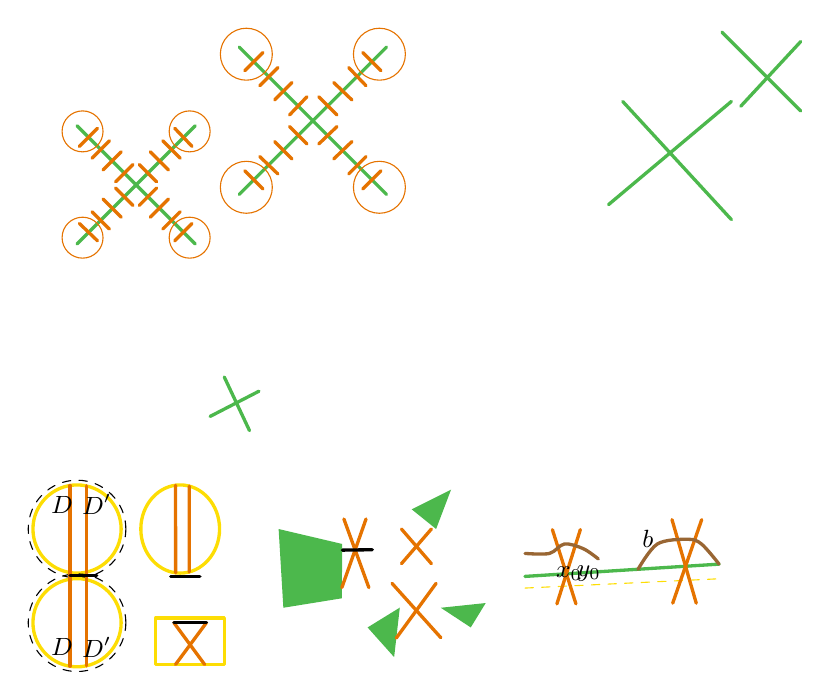
\begin{tikzpicture}[x=1mm,y=1mm,line cap=round,line join=round,font=\scriptsize]
\draw[Lg,very thick] (6.9,-11.9) -- (21.9,-26.9);
\draw[Lg,very thick] (6.9,-26.9) -- (21.9,-11.9);
\draw[Or,very thick] (14.8,-22) -- (17,-19.8);
\draw[Or,very thick] (14,-16.8) -- (11.8,-19);
\draw[Or,very thick] (17,-19) -- (14.8,-16.8);
\draw[Or,very thick] (11.8,-19.8) -- (14,-22);
\draw[Or,very thick] (16.2,-23.5) -- (18.5,-21.2);
\draw[Or,very thick] (12.5,-15.2) -- (10.2,-17.5);
\draw[Or,very thick] (18.5,-17.5) -- (16.2,-15.2);
\draw[Or,very thick] (10.2,-21.2) -- (12.5,-23.5);
\draw[Or,very thick] (17.8,-25) -- (20,-22.8);
\draw[Or,very thick] (11,-13.8) -- (8.8,-16);
\draw[Or,very thick] (20,-16) -- (17.8,-13.8);
\draw[Or,very thick] (8.8,-22.8) -- (11,-25);
\draw[Or,very thick] (19.3,-26.5) -- (21.5,-24.3);
\draw[Or,very thick] (9.5,-12.2) -- (7.2,-14.5);
\draw[Or,very thick] (21.5,-14.5) -- (19.3,-12.2);
\draw[Or,very thick] (7.2,-24.3) -- (9.5,-26.5);
\draw[Or] (23.8,-26.1) arc[start angle=0, end angle=360, x radius=2.6, y radius=2.6];
\draw[Or] (10.2,-12.6) arc[start angle=0, end angle=360, x radius=2.6, y radius=2.6];
\draw[Or] (23.8,-12.6) arc[start angle=0, end angle=360, x radius=2.6, y radius=2.6];
\draw[Or] (10.2,-26.1) arc[start angle=0, end angle=360, x radius=2.6, y radius=2.6];
\draw[Lg,very thick] (27.5,-1.9) -- (46.2,-20.6);
\draw[Lg,very thick] (27.5,-20.6) -- (46.2,-1.9);
\draw[Or,very thick] (37.6,-14.2) -- (39.9,-12);
\draw[Or,very thick] (36.1,-8.2) -- (33.9,-10.5);
\draw[Or,very thick] (39.9,-10.5) -- (37.6,-8.2);
\draw[Or,very thick] (33.9,-12) -- (36.1,-14.2);
\draw[Or,very thick] (39.5,-16.1) -- (41.8,-13.9);
\draw[Or,very thick] (34.2,-6.4) -- (32,-8.6);
\draw[Or,very thick] (41.8,-8.6) -- (39.5,-6.4);
\draw[Or,very thick] (32,-13.9) -- (34.2,-16.1);
\draw[Or,very thick] (41.4,-18) -- (43.6,-15.8);
\draw[Or,very thick] (32.4,-4.5) -- (30.1,-6.8);
\draw[Or,very thick] (43.6,-6.8) -- (41.4,-4.5);
\draw[Or,very thick] (30.1,-15.8) -- (32.4,-18);
\draw[Or,very thick] (43.2,-19.9) -- (45.5,-17.6);
\draw[Or,very thick] (30.5,-2.6) -- (28.2,-4.9);
\draw[Or,very thick] (45.5,-4.9) -- (43.2,-2.6);
\draw[Or,very thick] (28.2,-17.6) -- (30.5,-19.9);
\draw[Or] (48.6,-19.7) arc[start angle=0, end angle=360, x radius=3.3, y radius=3.3];
\draw[Or] (31.7,-2.8) arc[start angle=0, end angle=360, x radius=3.3, y radius=3.3];
\draw[Or] (48.6,-2.8) arc[start angle=0, end angle=360, x radius=3.3, y radius=3.3];
\draw[Or] (31.7,-19.7) arc[start angle=0, end angle=360, x radius=3.3, y radius=3.3];
\draw[Lg,very thick] (74.4,-21.9) -- (90,-8.8);
\draw[Lg,very thick] (76.2,-8.8) -- (90,-23.8);
\draw[Lg,very thick] (88.8,0) -- (98.8,-10);
\draw[Lg,very thick] (91.2,-9.4) -- (98.8,-1.2);
\draw[Lg,very thick] (23.8,-48.8) -- (30,-45.6);
\draw[Lg,very thick] (25.6,-43.8) -- (28.8,-50.6);
\draw[Ye,very thick] (6.9,-63.1) ellipse[x radius=5.6, y radius=5.6];
\draw[dashed] (6.9,-63.1) ellipse[x radius=6.2, y radius=6.2];
\draw[Ye,very thick] (6.9,-75) ellipse[x radius=5.6, y radius=5.6];
\draw[dashed] (6.9,-75) ellipse[x radius=6.2, y radius=6.2];
\draw[Or,very thick] (6.01,-57.57) -- (6.01,-80.53);
\draw[Or,very thick] (8.07,-57.62) -- (8.07,-80.48);
\draw[very thick] (6.01,-69) -- (9.4,-69);
\node[inner sep=1pt] at (5,-60) {\small $D$};
\node[inner sep=1pt] at (9.4,-60) {\small $D'$};
\node[inner sep=1pt] at (5,-78.1) {\small $D$};
\node[inner sep=1pt] at (9.4,-78.1) {\small $D'$};
\draw[Ye,very thick] (20,-63.1) ellipse[x radius=5, y radius=5.6];
\draw[Or,very thick] (19.41,-57.54) -- (19.42,-68.66);
\draw[Or,very thick] (21.16,-57.65) -- (21.14,-68.55);
\draw[very thick] (18.8,-69.1) -- (22.5,-69.1);
\draw[Ye,very thick] (16.9,-74.4) -- (25.6,-74.4) -- (25.6,-80.3) -- (16.9,-80.3) -- cycle;
\draw[Or,very thick] (19.2,-75) -- (23.1,-80.3);
\draw[Or,very thick] (23.33,-75) -- (19.41,-80.3);
\draw[very thick] (19.2,-75) -- (23.33,-75);
\fill[pattern=north east lines,Lg] (32.5,-63.1) -- (40.58,-65) -- (40.52,-71.9) -- (33.1,-73.1) -- cycle;
\fill[pattern=north east lines,Lg] (49.4,-60.6) -- (54.4,-58.1) -- (52.5,-63.1) -- cycle;
\fill[pattern=north east lines,Lg] (43.8,-75.6) -- (47.89,-73.08) -- (47.17,-79.37) -- cycle;
\fill[pattern=north east lines,Lg] (53.1,-73.1) -- (58.8,-72.5) -- (56.9,-75.6) -- cycle;
\draw[Or,very thick] (40.79,-61.83) -- (43.96,-70.54);
\draw[Or,very thick] (43.6,-61.83) -- (40.53,-70.54);
\draw[Or,very thick] (48.1,-63.1) -- (51.9,-67.5);
\draw[Or,very thick] (51.9,-63.1) -- (48.1,-67.5);
\draw[Or,very thick] (46.9,-70) -- (53.1,-76.9);
\draw[Or,very thick] (52.5,-70) -- (47.44,-76.95);
\draw[very thick] (40.6,-65.78) -- (44.4,-65.73);
\draw[Lg,very thick] (63.78,-69.12) -- (88.44,-67.56);
\draw[Ye,dashed] (63.8,-70.6) -- (88.8,-69.4);
\draw[Or,very thick] (67.27,-63.18) -- (70.26,-72.61);
\draw[Or,very thick] (70.82,-63.17) -- (67.84,-72.61);
\draw[Or,very thick] (82.46,-61.91) -- (85.54,-72.52);
\draw[Or,very thick] (86.23,-61.91) -- (82.55,-72.52);
\draw[Br,very thick] plot[smooth, tension=0.55] coordinates {(63.8,-66.2) (66.9,-66.2) (68.8,-65) (71.2,-65.6) (73.1,-66.9)};
\draw[Br,very thick] plot[smooth, tension=0.55] coordinates {(78.15,-68.21) (80.6,-65) (84.4,-64.4) (86.2,-65) (88.44,-67.56)};
\node[inner sep=1pt] at (79.4,-64.4) {\small $b$};
\node[inner sep=1pt] at (69.4,-68.8) {\small $x_0$};
\node[inner sep=1pt] at (71.9,-68.8) {\small $y_0$};
\end{tikzpicture}
\end{document}
